\section{1174087 - Ilham Muhammad Ariq}
\subsection{Teori}
\begin{enumerate}

	\item Jelaskan apa itu klasifikasi teks, sertakan gambar ilustrasi buatan sendiri.
	\hfill\break
	Klasifikasi teks merupakan sebuah model yang biasa digunakan untuk untuk mengkategorikan sebuah teks ke dalam kelompok-kelompok yang lebih terorganisir. Jadi untuk setiap kalimat yang di masukan ke dalam mesin, mesin tersebut akan menjadikan setiap kata dari kalimat tersebut menjadi sebuah kolom. Untuk ilustrasinya bisa dilihat pada gambar berikut 

	\begin{figure}[H]
	\centering
		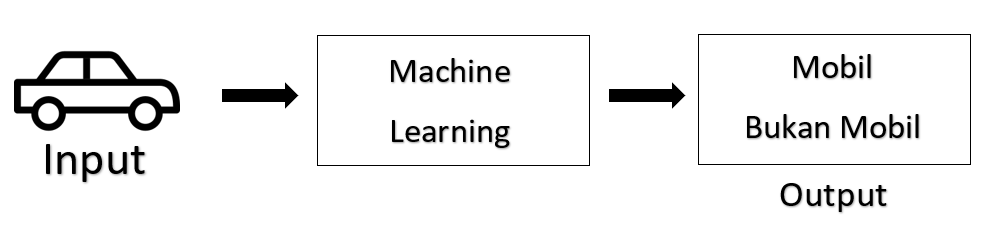
\includegraphics[width=7cm]{figures/1174087/4/1.png}
		\caption{Klasifikasi teks}
	\end{figure}
	
	\item Jelaskan mengapa Klasifikasi bunga tidak bisa menggunakan machine learning, sertakan ilustrasi sendiri.	
	\hfill\break
	Karena machine learning tidak dapat menampilkan inputan sesuai dengan apa yang kita inputkan. Karena inputan tersebut serupa namun mesin memberikan output yang berbeda, biasanya output atau error ini disebut dengan istilah noise. Untuk contoh sederhananya misalkan kita inputkan salah satu label yang terdapat pada bunga, output yang dihasilkan oleh mesin tersebut ialah label yang lain. Itu dikarenakan bunga banyak jenis yang serupa namun bentuk dan ukurannya tidak sama. Untuk ilustrasinya bisa dilihat pada gambar berikut 

	\begin{figure}[H]
	\centering
		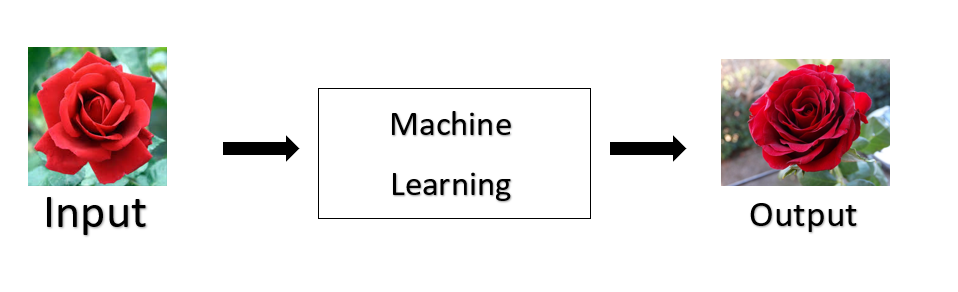
\includegraphics[width=7cm]{figures/1174087/4/2.png}
		\caption{Klasifikasi Bunga}
	\end{figure}

	\item Jelaskan bagaimana teknik pembelajaran mesin pada teks pada kata-kata yang digunakan di youtube,jelaskan arti per atribut data csv dan sertakan ilustrasi buatan sendiri.

	Teknik machine learning yang dipakai pada teks yang digunakan di youtube bisa menggunakan bag of words dan random forest. Bag of words adalah proses mengubah teks menjadi vektor dengan panjang tetap dengan cara menghitung berapa kali setiap kata itu muncul. Random forest (RF) adalah suatu algoritma yang digunakan pada klasifikasi data dalam jumlah yang besar. Klasifikasi random forest dilakukan melalui penggabungan pohon (tree) dengan melakukan training pada sampel data yang dimiliki.\\
	Atribut yang ada pada file csv Youtube01-Psy diantaranya, COMMENT\_ID, AUTHOR, DATE, CONTENT, CLASS.
	\begin{itemize}
		\item COMMENT\_ID : merupakan key unik yang membedakan komen lainnya.
		\item AUTHOR : merupakan penulis dari komen tersebut.
		\item DATE : merupakan waktu dari komen tersebut dipublikasikan.
		\item CONTENT : merupakan isi komentarnya.
		\item CLASS : merupakan klasifikasi dari komennya (spam/notspam).
	\end{itemize}

	\item Jelaskan apa yang dimaksud vektorisasi data.
	\hfill\break
	Vektorisasi data ialah suatu pemecahan atau pembagian data berupa teks, sebagai contoh terdapat 5 paragraf, data teks tersebut di pecah menjadi kalimat-kalimat yang lebih sederhana, lalu di pecah lagi menjadi kata untuk setiap kalimatnya. 

	\item Jelaskan apa yang dimaksud dengan bag of words dengan ilustrasi sendiri.
	\hfill\break
	Bag of words adalah representasi penyederhanaan sebuah kalimat atau perhitungan setiap kata pada suatu kalimat dengan presentase berapa kali muncul kata tersebut untuk setiap kalimatnya. Contoh ilustrasi sederhananya seperti berikut 

	\begin{figure}[H]
	\centering
		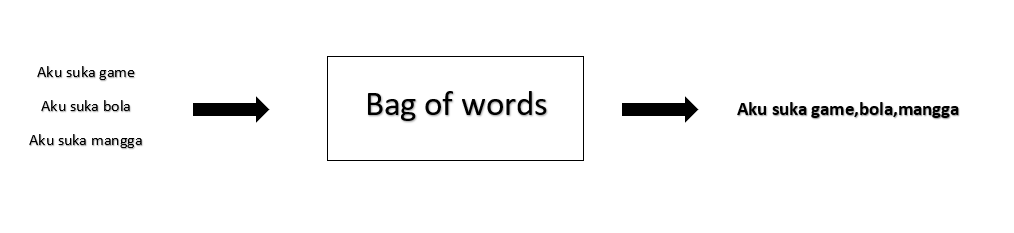
\includegraphics[width=7cm]{figures/1174087/4/3.png}
		\caption{Bag of words}
	\end{figure}

	\item Jelaskan apa yang dimaksud dengan TF-IDF.
	\hfill\break
	TF-IDF merupakan metode untuk menghitung bobot setiap kata pada suatu kalimat yang paling sering digunakan. TF-IDF ini akan menghitung nilai Term Frequency dan Inverse Document Frequency pada setiap kata dalam setiap kalimat yang muncul dengan diimbangi dengan jumlah dokumen dalam korpus yang mengandung kata. Contoh ilustrasi sederhananya seperti gambar berikut 

	\begin{figure}[H]
	\centering
		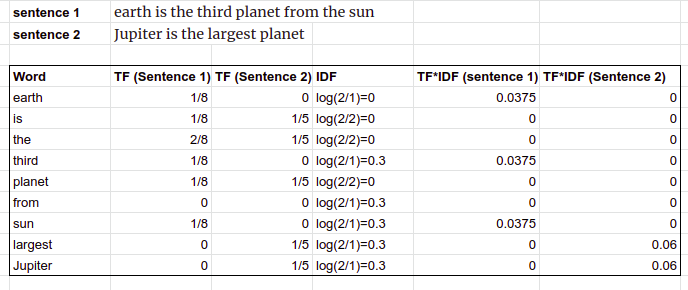
\includegraphics[width=7cm]{figures/1174087/4/4.png}
		\caption{TF-IDF}
	\end{figure}
\end{enumerate}


\subsection{Praktek Program}
\begin{enumerate}
	\item Soal 1
	\hfill\break
	\lstinputlisting[firstline=9, lastline=10]{src/1174087/4/1174087.py}
	Kode di atas digunakan untuk buat aplikasi sederhana menggunakan pandas dengan format csv sebanyak 500 baris, hasilnya ialah sebagai berikut  
	\begin{figure}[H]
	\centering
		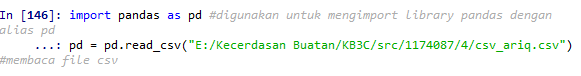
\includegraphics[width=5cm]{figures/1174087/4/5.png}
		\caption{Soal 1}
	\end{figure}

	\item Soal 2
	\hfill\break
	\lstinputlisting[firstline=13, lastline=14]{src/1174087/4/1174087.py}
	Kode di atas digunakan untuk memecah dataframe tersebut menjadi dua bagian yaitu 450 row pertama dan 50 row kedua. Hasilnya adalah sebagai berikut 
	\begin{figure}[H]
	\centering
		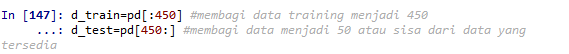
\includegraphics[width=4cm]{figures/1174087/4/6.png}
		\caption{Soal 2}
	\end{figure}

	\item Soal 3
	\hfill\break
	\lstinputlisting[firstline=17, lastline=40]{src/1174087/4/1174087.py}
	Dengan menggunakan 1174087 mod 4 adalah 3, yang artinya menggunakan dataset shakira. Hasilnya adalah sebagai berikut 
	\begin{figure}[H]
	\centering
		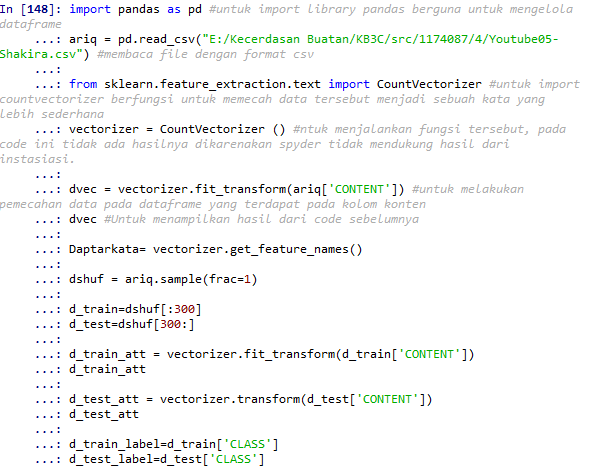
\includegraphics[width=5cm]{figures/1174087/4/7.png}
		\caption{Soal 3}
	\end{figure}

	\item Soal 4
	\hfill\break
	\lstinputlisting[firstline=44, lastline=46]{src/1174087/4/1174087.py}
	Klasifikasi dari data vektorisasi menggunakan klasifikasi SVM. Hasilnya adalah sebagai berikut 
	\begin{figure}[H]
	\centering
		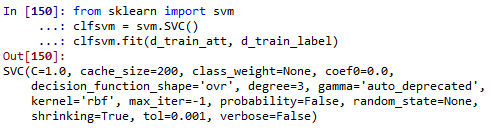
\includegraphics[width=5cm]{figures/1174087/4/8.png}
		\caption{Soal 4}
	\end{figure}

	\item Soal 5
	\hfill\break
	\lstinputlisting[firstline=50, lastline=52]{src/1174087/4/1174087.py}
	Klasifikasi dari data vektorisasi menggunakan klasifikasi Decision Tree. Hasilnya adalah sebagai berikut 
	
	\begin{figure}[H]
	\centering
		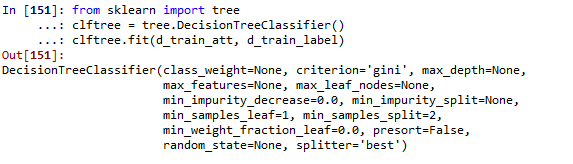
\includegraphics[width=5cm]{figures/1174087/4/9.png}
		\caption{Soal 5}
	\end{figure}

	\item Soal 6
	\hfill\break
	\lstinputlisting[firstline=55, lastline=72]{src/1174087/4/1174087.py}
	Plot confusion matrix dari praktik modul ini menggunakan matplotlib. Hasilnya adalah sebagai berikut 
	\begin{figure}[H]
	\centering
		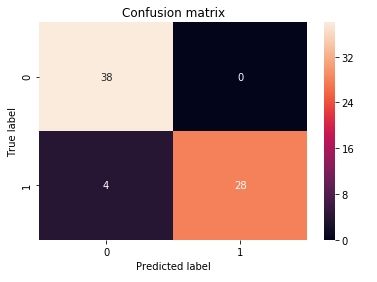
\includegraphics[width=5cm]{figures/1174087/4/10.png}
		\caption{Soal 6}
	\end{figure}

	\item Soal 7
	\hfill\break
	\lstinputlisting[firstline=75, lastline=79]{src/1174087/4/1174087.py}
	Menjalankan program cross validation. Hasilnya adalah sebagai berikut 
	\begin{figure}[H]
	\centering
		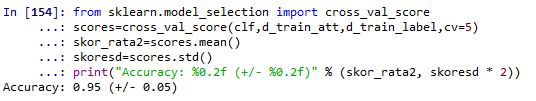
\includegraphics[width=5cm]{figures/1174087/4/11.png}
		\caption{Soal 7}
	\end{figure}

	\item Soal 8
	\hfill\break
	\lstinputlisting[firstline=82, lastline=97]{src/1174087/4/1174087.py}
	Program pengamatan komponen informasi. Jadi disini kita akan memprediksi nilai dari variabel test att dan test pass Hasilnya adalah sebagai berikut 
	\begin{figure}[H]
	\centering
		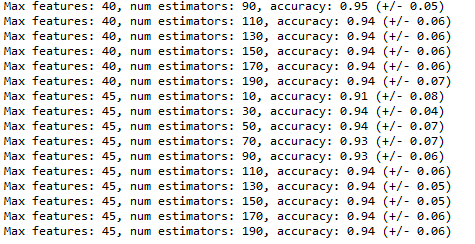
\includegraphics[width=5cm]{figures/1174087/4/12.png}
		\caption{Soal 8}
	\end{figure}
\end{enumerate}

\subsection{Penanganan Error}
\begin{enumerate}
	\item ScreenShoot Error
	\begin{figure}[H]
		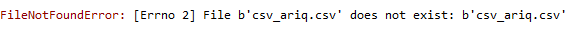
\includegraphics[width=5cm]{figures/1174087/4/error.png}
		\centering
		\caption{FileNotFoundError}
	\end{figure}
	\item Cara Penangan Error
	\begin{itemize}
		\item FileNotFoundError
		\hfill\break
		Dengan menyesuaikan letak file csv pada codingannya, sehingga dapat  di baca atau dipanggil file csvnya.
	\end{itemize}
\end{enumerate}

\subsection{Bukti Tidak Plagiat}
\begin{figure}[H]
\centering
	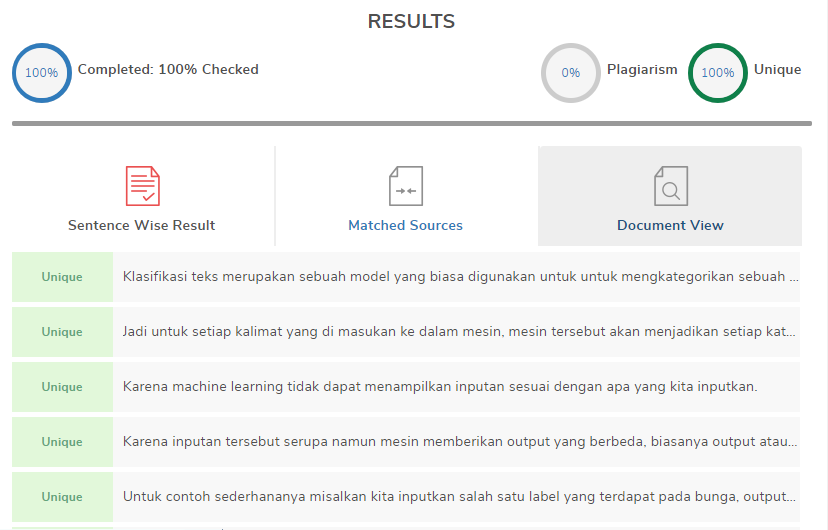
\includegraphics[width=4cm]{figures/1174087/4/plagiat.png}
	\caption{Bukti Tidak Melakukan Plagiat Chapter 4}
\end{figure}

\subsection{Link Youtube}
https://youtu.be/lLxUddy2kW4